% Generated by tools/plot_tikz.py -- do not edit by hand.
% Needs \usepackage{tikz}; no TikZ libraries required.
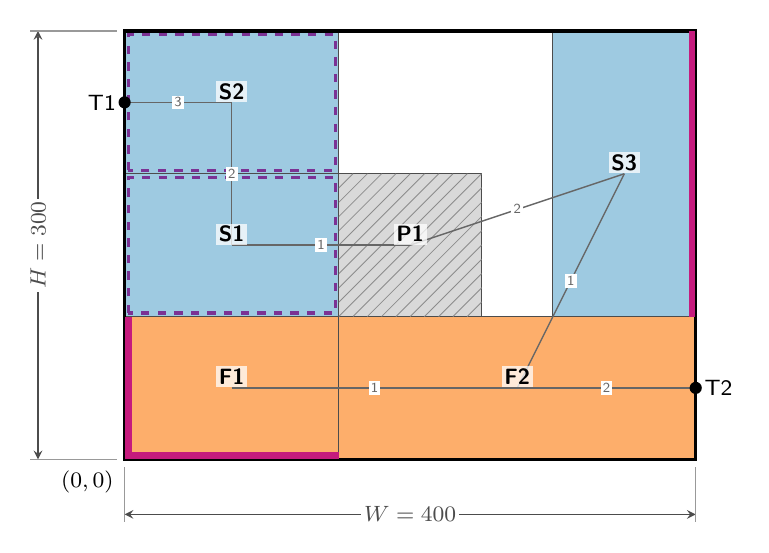
\begin{tikzpicture}[x=0.0015\textwidth,y=0.0015\textwidth,font=\sffamily]
\definecolor{lab3soft}{HTML}{9ECAE1}
\definecolor{lab3fixed}{HTML}{FDAE6B}
\definecolor{lab3preplaced}{HTML}{D9D9D9}
\definecolor{lab3mib0}{HTML}{7B3294}
\definecolor{lab3mib1}{HTML}{008837}
\definecolor{lab3mib2}{HTML}{E66101}
\definecolor{lab3mib3}{HTML}{0571B0}
\definecolor{lab3mib4}{HTML}{CA0020}
\definecolor{lab3mib5}{HTML}{5E3C99}
\definecolor{lab3mib6}{HTML}{1B7837}
\definecolor{lab3mib7}{HTML}{B35806}
\definecolor{lab3mib8}{HTML}{2166AC}
\definecolor{lab3mib9}{HTML}{D6604D}
\definecolor{lab3mib10}{HTML}{542788}
\definecolor{lab3mib11}{HTML}{01665E}
\definecolor{lab3bound}{HTML}{C51B7D}
\fill[white] (0,0) rectangle (400,300);
\filldraw[fill=lab3soft,draw=black!70,line width=0.4pt] (0,100) rectangle (150,200);
\filldraw[fill=lab3soft,draw=black!70,line width=0.4pt] (0,200) rectangle (150,300);
\filldraw[fill=lab3soft,draw=black!70,line width=0.4pt] (300,100) rectangle (400,300);
\filldraw[fill=lab3fixed,draw=black!70,line width=0.4pt] (0,0) rectangle (150,100);
\filldraw[fill=lab3fixed,draw=black!70,line width=0.4pt] (150,0) rectangle (400,100);
\filldraw[fill=lab3preplaced,draw=black!70,line width=0.4pt] (150,100) rectangle (250,200);
\begin{scope}
\clip (150,100) rectangle (250,200);
\draw[black!45,line width=0.3pt] (50,100) -- (150,200);
\draw[black!45,line width=0.3pt] (60,100) -- (160,200);
\draw[black!45,line width=0.3pt] (70,100) -- (170,200);
\draw[black!45,line width=0.3pt] (80,100) -- (180,200);
\draw[black!45,line width=0.3pt] (90,100) -- (190,200);
\draw[black!45,line width=0.3pt] (100,100) -- (200,200);
\draw[black!45,line width=0.3pt] (110,100) -- (210,200);
\draw[black!45,line width=0.3pt] (120,100) -- (220,200);
\draw[black!45,line width=0.3pt] (130,100) -- (230,200);
\draw[black!45,line width=0.3pt] (140,100) -- (240,200);
\draw[black!45,line width=0.3pt] (150,100) -- (250,200);
\draw[black!45,line width=0.3pt] (160,100) -- (260,200);
\draw[black!45,line width=0.3pt] (170,100) -- (270,200);
\draw[black!45,line width=0.3pt] (180,100) -- (280,200);
\draw[black!45,line width=0.3pt] (190,100) -- (290,200);
\draw[black!45,line width=0.3pt] (200,100) -- (300,200);
\draw[black!45,line width=0.3pt] (210,100) -- (310,200);
\draw[black!45,line width=0.3pt] (220,100) -- (320,200);
\draw[black!45,line width=0.3pt] (230,100) -- (330,200);
\draw[black!45,line width=0.3pt] (240,100) -- (340,200);
\end{scope}
\draw[lab3mib0,dashed,line width=1.2pt] (2.5,102.5) rectangle (147.5,197.5);
\draw[lab3mib0,dashed,line width=1.2pt] (2.5,202.5) rectangle (147.5,297.5);
\draw[black!60,line width=0.5pt] (75,150) -- node[fill=white,inner sep=0.8pt,font=\sffamily\tiny] {2} (75,250);
\draw[black!60,line width=0.5pt] (75,150) -- node[fill=white,inner sep=0.8pt,font=\sffamily\tiny] {1} (200,150);
\draw[black!60,line width=0.5pt] (75,250) -- node[fill=white,inner sep=0.8pt,font=\sffamily\tiny] {3} (0,250);
\draw[black!60,line width=0.5pt] (200,150) -- node[fill=white,inner sep=0.8pt,font=\sffamily\tiny] {2} (350,200);
\draw[black!60,line width=0.5pt] (75,50) -- node[fill=white,inner sep=0.8pt,font=\sffamily\tiny] {1} (275,50);
\draw[black!60,line width=0.5pt] (275,50) -- node[fill=white,inner sep=0.8pt,font=\sffamily\tiny] {2} (400,50);
\draw[black!60,line width=0.5pt] (350,200) -- node[fill=white,inner sep=0.8pt,font=\sffamily\tiny] {1} (275,50);
\node[font=\sffamily\footnotesize\bfseries,fill=white,fill opacity=0.75,text opacity=1,inner sep=1pt,above] at (75,150) {S1};
\node[font=\sffamily\footnotesize\bfseries,fill=white,fill opacity=0.75,text opacity=1,inner sep=1pt,above] at (75,250) {S2};
\node[font=\sffamily\footnotesize\bfseries,fill=white,fill opacity=0.75,text opacity=1,inner sep=1pt,above] at (350,200) {S3};
\node[font=\sffamily\footnotesize\bfseries,fill=white,fill opacity=0.75,text opacity=1,inner sep=1pt,above] at (75,50) {F1};
\node[font=\sffamily\footnotesize\bfseries,fill=white,fill opacity=0.75,text opacity=1,inner sep=1pt,above] at (275,50) {F2};
\node[font=\sffamily\footnotesize\bfseries,fill=white,fill opacity=0.75,text opacity=1,inner sep=1pt,above] at (200,150) {P1};
\draw[black,line width=1.2pt] (0,0) rectangle (400,300);
\draw[lab3bound,line width=2.4pt,line cap=butt] ([xshift=1.3pt]0,0) -- ([xshift=1.3pt]0,100);
\draw[lab3bound,line width=2.4pt,line cap=butt] ([yshift=1.3pt]0,0) -- ([yshift=1.3pt]150,0);
\draw[lab3bound,line width=2.4pt,line cap=butt] ([xshift=-1.3pt]400,100) -- ([xshift=-1.3pt]400,300);
\fill[black] (0,250) circle (2.2pt);
\node[anchor=east,font=\sffamily\footnotesize,inner sep=3pt] at (0,250) {T1};
\fill[black] (400,50) circle (2.2pt);
\node[anchor=west,font=\sffamily\footnotesize,inner sep=3pt] at (400,50) {T2};
\draw[black!70,<->,>=stealth] ([yshift=-7mm]0,0) -- node[fill=white,inner sep=1pt,font=\sffamily\footnotesize] {$W=400$} ([yshift=-7mm]400,0);
\draw[black!40] ([yshift=-1mm]0,0) -- ([yshift=-8mm]0,0);
\draw[black!40] ([yshift=-1mm]400,0) -- ([yshift=-8mm]400,0);
\draw[black!70,<->,>=stealth] ([xshift=-11mm]0,0) -- node[fill=white,inner sep=1pt,font=\sffamily\footnotesize,rotate=90] {$H=300$} ([xshift=-11mm]0,300);
\draw[black!40] ([xshift=-1mm]0,0) -- ([xshift=-12mm]0,0);
\draw[black!40] ([xshift=-1mm]0,300) -- ([xshift=-12mm]0,300);
\node[anchor=north east,font=\sffamily\footnotesize,inner sep=1pt] at ([xshift=-1mm,yshift=-1mm]0,0) {$(0,0)$};
\end{tikzpicture}
